\documentclass[10pt,aspectratio=169,serif]{beamer}

\usepackage[fontset=none, scheme=plain]{ctex}
\IfFontExistsTF{Songti SC}{%
	\setCJKmainfont{Songti SC}[AutoFakeSlant=0.2]%
	\setCJKsansfont{Songti SC}[AutoFakeSlant=0.2]%
}{%
	\setCJKmainfont{FandolSong-Regular}[Extension=.otf,BoldFont=FandolSong-Bold,AutoFakeSlant=0.2]%
	\setCJKsansfont{FandolSong-Regular}[Extension=.otf,BoldFont=FandolSong-Bold]%
}
\usepackage{amsmath,amssymb,graphicx,tikz,booktabs,multicol,calligra}
\usepackage{pgfplots}
\pgfplotsset{compat=1.18}
\usepackage{tcolorbox}
\tcbuselibrary{skins}
\usepackage{XyygU}
\usepackage{caption}
\captionsetup[figure]{name=图,labelsep=period}

\usetikzlibrary{arrows.meta,positioning,calc}

\setlength{\abovedisplayskip}{0pt plus 2pt minus 2pt}
\setlength{\belowdisplayskip}{0pt plus 2pt minus 2pt}

\title[习题5.6]{习题5.6 函数 $y=A\sin(\omega x+\varphi)$}
\subtitle{复习巩固 \& 综合运用}
\author{}
\institute{}
\date{2026-10-16}

\begin{document}

\begin{frame}
  \titlepage
\end{frame}

% --- 1 ---
\begin{frame}[t]{第1题：选择题（余弦曲线的变换）}
\textbf{1.} 选择题：
\begin{enumerate}
  \item 为得到 $y=\cos\!\left(x+\dfrac13\right)$ 的图象，只需把余弦曲线上所有的点（\quad）。
  \item 为得到 $y=\cos\dfrac{x}{5}$ 的图象，只需把余弦曲线上所有的点（\quad）。
  \item 为得到 $y=\dfrac14\cos x$ 的图象，只需把余弦曲线上所有的点（\quad）。
\end{enumerate}
\end{frame}

\begin{frame}[t]{第1题 解答}
\begin{tcolorbox}[colback=orange!10,colframe=orange,title=\textbf{解}]
(1) $x+\dfrac13$ 是平移变换，注意此处是弧度 $\dfrac13$（不是 $\dfrac{\pi}{3}$）。向左平移 $\dfrac13$ 个单位长度。\alert{选 (C)}。

(2) $\cos\dfrac{x}{5}$ 即 $\omega=\dfrac15<1$，横坐标伸长到原来的 $5$ 倍，纵坐标不变。\alert{选 (A)}。

(3) $\dfrac14\cos x$ 即振幅变为 $\dfrac14$，纵坐标缩短到原来的 $\dfrac14$，横坐标不变。\alert{选 (D)}。
\end{tcolorbox}
\end{frame}

% --- 2 ---
\begin{frame}[t]{第2题：画简图}
\textbf{2.} 画出下列函数在长度为一个周期的闭区间上的简图：
\begin{enumerate}
  \item $y=4\sin\dfrac12 x$；\qquad
  \item $y=\dfrac12\cos 3x$；
  \item $y=3\sin\!\left(2x+\dfrac{\pi}{6}\right)$；\qquad
  \item $y=2\cos\!\left(\dfrac12 x-\dfrac{\pi}{4}\right)$。
\end{enumerate}
\end{frame}

\begin{frame}[t]{第2题 解答：(1) $y=4\sin\frac12 x$}
\begin{tcolorbox}[colback=orange!10,colframe=orange,title=\textbf{解}]
振幅 $4$，周期 $T=\dfrac{2\pi}{1/2}=4\pi$，初相 $0$。
\end{tcolorbox}
\begin{center}
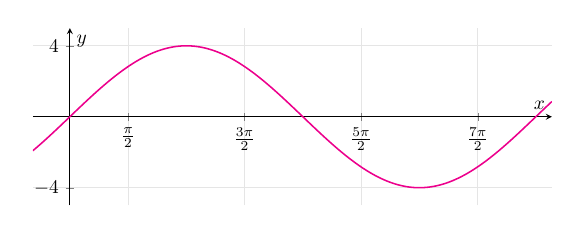
\begin{tikzpicture}[scale=0.7]
\begin{axis}[width=11cm,height=4.8cm,axis lines=middle,xlabel=$x$,ylabel=$y$,
xmin=-1,xmax=13,ymin=-5,ymax=5,xtick={1.57,4.71,7.85,11},xticklabels={$\frac{\pi}{2}$,$\frac{3\pi}{2}$,$\frac{5\pi}{2}$,$\frac{7\pi}{2}$},
ytick={-4,4},grid=major,grid style={gray!20}]
\addplot[thick,magenta,domain=-1:13,samples=200] {4*sin(deg(0.5*x))};
\end{axis}
\end{tikzpicture}
\end{center}
\end{frame}

\begin{frame}[t]{第2题 解答：(2) $y=\frac12\cos 3x$}
\begin{tcolorbox}[colback=orange!10,colframe=orange,title=\textbf{解}]
振幅 $\frac12$，周期 $T=\dfrac{2\pi}{3}$。
\end{tcolorbox}
\begin{center}
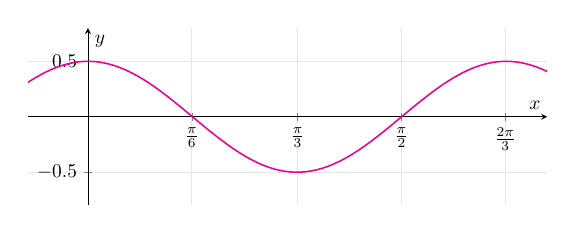
\begin{tikzpicture}[scale=0.7]
\begin{axis}[width=11cm,height=4.8cm,axis lines=middle,xlabel=$x$,ylabel=$y$,
xmin=-0.3,xmax=2.3,ymin=-0.8,ymax=0.8,xtick={0.52,1.05,1.57,2.09},xticklabels={$\frac{\pi}{6}$,$\frac{\pi}{3}$,$\frac{\pi}{2}$,$\frac{2\pi}{3}$},
ytick={-0.5,0.5},grid=major,grid style={gray!20}]
\addplot[thick,magenta,domain=-0.3:2.3,samples=200] {0.5*cos(deg(3*x))};
\end{axis}
\end{tikzpicture}
\end{center}
\end{frame}

\begin{frame}[t]{第2题 解答：(3) $y=3\sin(2x+\frac{\pi}{6})$}
\begin{tcolorbox}[colback=orange!10,colframe=orange,title=\textbf{解}]
振幅 $3$，周期 $T=\pi$，$2x+\dfrac{\pi}{6}=0$ 时 $x=-\dfrac{\pi}{12}$。
\end{tcolorbox}
\begin{center}
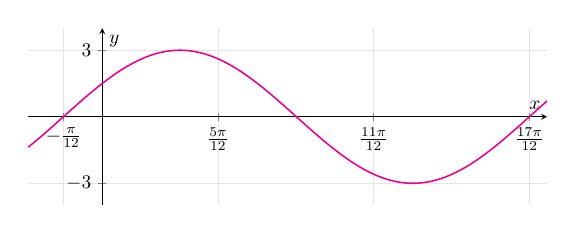
\begin{tikzpicture}[scale=0.7]
\begin{axis}[width=11cm,height=4.8cm,axis lines=middle,xlabel=$x$,ylabel=$y$,
xmin=-0.5,xmax=3,ymin=-4,ymax=4,xtick={-0.26,0.78,1.83,2.88},xticklabels={$-\frac{\pi}{12}$,$\frac{5\pi}{12}$,$\frac{11\pi}{12}$,$\frac{17\pi}{12}$},
ytick={-3,3},grid=major,grid style={gray!20}]
\addplot[thick,magenta,domain=-0.5:3,samples=200] {3*sin(deg(2*x+pi/6))};
\end{axis}
\end{tikzpicture}
\end{center}
\end{frame}

\begin{frame}[t]{第2题 解答：(4) $y=2\cos(\frac12 x-\frac{\pi}{4})$}
\begin{tcolorbox}[colback=orange!10,colframe=orange,title=\textbf{解}]
振幅 $2$，周期 $T=4\pi$。
\end{tcolorbox}
\begin{center}
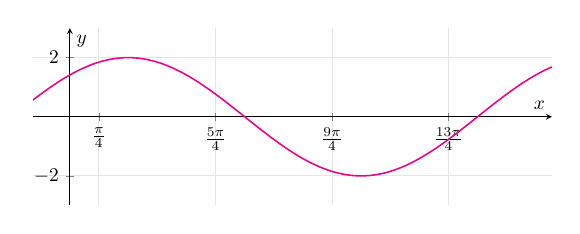
\begin{tikzpicture}[scale=0.7]
\begin{axis}[width=11cm,height=4.8cm,axis lines=middle,xlabel=$x$,ylabel=$y$,
xmin=-1,xmax=13,ymin=-3,ymax=3,xtick={0.78,3.93,7.07,10.21},xticklabels={$\frac{\pi}{4}$,$\frac{5\pi}{4}$,$\frac{9\pi}{4}$,$\frac{13\pi}{4}$},
ytick={-2,2},grid=major,grid style={gray!20}]
\addplot[thick,magenta,domain=-1:13,samples=200] {2*cos(deg(0.5*x-pi/4))};
\end{axis}
\end{tikzpicture}
\end{center}
\end{frame}

% --- 3 ---
\begin{frame}[t]{第3题：由正弦曲线变换（注意定义域）}
\textbf{3.} 说明下列函数的图象可由正弦曲线经过怎样的变换得到（注意定义域）：
\begin{enumerate}
  \item $y=8\sin\!\left(\dfrac{x}{4}-\dfrac{\pi}{8}\right)$，$x\in[0,+\infty)$；
  \item $y=\dfrac13\sin\!\left(3x+\dfrac{\pi}{7}\right)$，$x\in[0,+\infty)$。
\end{enumerate}
\end{frame}

\begin{frame}[t]{第3题 解答}
\begin{tcolorbox}[colback=orange!10,colframe=orange,title=\textbf{解}]
(1) 由 $y=\sin x$：
\begin{itemize}
  \item 向右平移 $\dfrac{\pi}{8}$，得 $y=\sin\!\left(x-\dfrac{\pi}{8}\right)$；
  \item 横坐标伸长到原来的 $4$ 倍，得 $y=\sin\!\left(\dfrac{x}{4}-\dfrac{\pi}{8}\right)$；
  \item 纵坐标伸长到原来的 $8$ 倍；
  \item 取 $x\ge 0$ 的部分。
\end{itemize}
周期 $T=8\pi$。

(2) 由 $y=\sin x$：
\begin{itemize}
  \item 向左平移 $\dfrac{\pi}{7}$，得 $y=\sin\!\left(x+\dfrac{\pi}{7}\right)$；
  \item 横坐标缩短到原来的 $\dfrac13$，得 $y=\sin\!\left(3x+\dfrac{\pi}{7}\right)$；
  \item 纵坐标缩短到原来的 $\dfrac13$；
  \item 取 $x\ge 0$ 的部分。
\end{itemize}
周期 $T=\dfrac{2\pi}{3}$。
\end{tcolorbox}
\end{frame}

% --- 4 ---
\begin{frame}[t]{第4题：由图象求解析式}
\textbf{4.} 函数 $y=A\sin(\omega x+\varphi)$（$A>0,\omega>0,0<\varphi<\pi$）在一个周期内的图象如图所示，求此函数的解析式。

\begin{center}
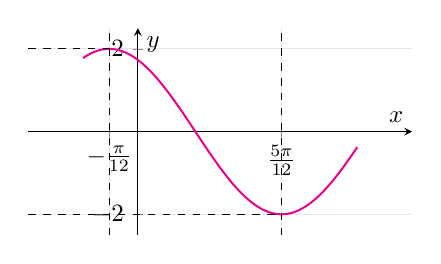
\begin{tikzpicture}[scale=0.9]
\begin{axis}[width=7cm,height=4.5cm,axis lines=middle,xlabel=$x$,ylabel=$y$,
xmin=-1,xmax=2.5,ymin=-2.5,ymax=2.5,
xtick={-0.262,1.309},xticklabels={$-\frac{\pi}{12}$,$\frac{5\pi}{12}$},
ytick={-2,2},grid=major,grid style={gray!20}]
\addplot[thick,magenta,domain=-0.5:2,samples=100] {2*sin(deg(2*x+2*pi/3))};
\draw[dashed] (axis cs:-0.262,-2.5) -- (axis cs:-0.262,2.5);
\draw[dashed] (axis cs:1.309,-2.5) -- (axis cs:1.309,2.5);
\draw[dashed] (axis cs:-1,2) -- (axis cs:-0.262,2);
\draw[dashed] (axis cs:-1,-2) -- (axis cs:1.309,-2);
\end{axis}
\end{tikzpicture}
\end{center}
\end{frame}

\begin{frame}[t]{第4题 解答}
\begin{tcolorbox}[colback=orange!10,colframe=orange,title=\textbf{解}]
由图知振幅 $A=2$。
最高点在 $x=-\dfrac{\pi}{12}$，最低点在 $x=\dfrac{5\pi}{12}$，两者相差半个周期：
\[
\frac{T}{2}=\frac{5\pi}{12}-\!\left(-\frac{\pi}{12}\right)=\frac{\pi}{2}\ \Longrightarrow\ T=\pi,\ \omega=2.
\]
最高点处相位为 $\dfrac{\pi}{2}$：
\[
2\cdot\!\left(-\frac{\pi}{12}\right)+\varphi=\frac{\pi}{2}\ \Longrightarrow\ \varphi=\frac{2\pi}{3}.
\]
\alert{$y=2\sin\!\left(2x+\dfrac{2\pi}{3}\right)$}。
\end{tcolorbox}
\end{frame}

% --- 5 ---
\begin{frame}[t]{第5题：平移后求 $g(x)$}
\textbf{5.} 将函数 $y=3\sin\!\left(2x+\dfrac{\pi}{4}\right)$ 的图象向左平移 $\dfrac{\pi}{3}$ 后得到函数 $y=g(x)$ 的图象，求 $y=g(x)$ 的解析式。
\end{frame}

\begin{frame}[t]{第5题 解答}
\begin{tcolorbox}[colback=orange!10,colframe=orange,title=\textbf{解}]
左移 $\dfrac{\pi}{3}$，即将 $x$ 替换为 $x+\dfrac{\pi}{3}$：
\[
g(x)=3\sin\!\left[2\!\left(x+\frac{\pi}{3}\right)+\frac{\pi}{4}\right]
=3\sin\!\left(2x+\frac{2\pi}{3}+\frac{\pi}{4}\right)
=3\sin\!\left(2x+\frac{11\pi}{12}\right).
\]
\end{tcolorbox}
\end{frame}

% --- 6 ---
\begin{frame}[t]{第6题：秒针端点距离}
\textbf{6.} 某时钟的秒针端点 $A$ 到中心点 $O$ 的距离为 $5$ cm，秒针绕点 $O$ 匀速旋转，当时间 $t=0$ 时，点 $A$ 与钟面上标 $12$ 的点 $B$ 重合。将 $A$，$B$ 两点间的距离 $d$（单位：cm）表示成 $t$（单位：s）的函数，则 $d=$ \underline{\hspace{2cm}}，$t\in[0,60]$。
\end{frame}

\begin{frame}[t]{第6题 解答}
\begin{tcolorbox}[colback=orange!10,colframe=orange,title=\textbf{解}]
秒针周期 $60$ s，角速度 $\omega=\dfrac{2\pi}{60}=\dfrac{\pi}{30}$ rad/s。
$t$ 秒后，$OA$ 与 $OB$ 的夹角 $\theta=\omega t=\dfrac{\pi t}{30}$。
在等腰 $\triangle OAB$ 中，$OA=OB=5$，由弦长公式：
\[
d=2\cdot 5\cdot\sin\frac{\theta}{2}=10\sin\frac{\pi t}{60}.
\]
\alert{$d=10\sin\dfrac{\pi t}{60}$，$t\in[0,60]$}。
\end{tcolorbox}
\end{frame}

% --- 7 ---
\begin{frame}[t]{第7题：筒车问题}
\textbf{7.} 一个半径为 $3$ m 的筒车按逆时针方向每分转 $1.5$ 圈，轴心 $O$ 距水面 $2.2$ m。盛水筒 $P$ 到水面距离 $d$（水面下为负），$P$ 刚浮出水面时开始计时，$d=A\sin(\omega t+\varphi)+K$（$A>0,\omega>0,-\frac{\pi}{2}<\varphi<\frac{\pi}{2}$）。
\begin{enumerate}
  \item 求 $A,\omega,\varphi,K$（$\varphi$ 精确到 $0.0001$）；
  \item 盛水筒出水后至少经过多长时间可到达最高点（精确到 $0.01$ s）？
\end{enumerate}
\end{frame}

\begin{frame}[t]{第7题 解答}
\begin{tcolorbox}[colback=orange!10,colframe=orange,title=\textbf{解}]
(1) $A=3$（半径）；$K=2.2$（轴心距水面高度）。
每分钟 $1.5$ 圈，$\omega=\dfrac{1.5\times 2\pi}{60}=\dfrac{\pi}{20}$ rad/s。

$t=0$ 时 $d=0$，且开始向上运动：
\[
3\sin\varphi+2.2=0\ \Longrightarrow\ \sin\varphi=-\frac{2.2}{3}=-\frac{11}{15}.
\]
上升要求 $\cos\varphi>0$，故 $\varphi=-\arcsin\dfrac{11}{15}\approx -0.8230$。

(2) 最高点 $d=5.2$ 即 $\sin(\omega t+\varphi)=1$：
\[
\omega t+\varphi=\frac{\pi}{2}\ \Longrightarrow\ t=\frac{\pi/2-\varphi}{\omega}=\frac{\pi/2+0.8230}{\pi/20}\approx 15.24\ \text{s}.
\]
\end{tcolorbox}
\end{frame}

\begin{frame}[c]
  \begin{center}
    {\Huge\calligra Thanks!}
  \end{center}
\end{frame}

\end{document}
